\documentclass[12pt]{article}
\usepackage[top=2in, bottom=1.5in, left=1in, right=1in]{geometry}
\usepackage{pdfpages}
\usepackage{fancyhdr}
\usepackage{pgfplots}
\usepackage{listings}
\usepackage{hyperref}
\usepackage{menukeys}
\usepackage{tabularx}
\usepackage[T1]{fontenc}
\usepackage{graphicx}
\graphicspath{ {images/} }
\usepackage{listings}
\lstdefinelanguage{diff}{
  morecomment=[f][\color{blue}]{@@},     % group identifier
  morecomment=[f][\color{red}]-,         % deleted lines 
  morecomment=[f][\color{green}]+,       % added lines
  morecomment=[f][\color{magenta}]{---}, % Diff header lines (must appear after +,-)
  morecomment=[f][\color{magenta}]{+++},
}
\lstdefinelanguage{javascript}{
  keywords={typeof, new, true, false, catch, function, return, null, catch, switch, var, if, in, while, do, else, case, break},
  keywordstyle=\color{blue}\bfseries,
  ndkeywords={class, export, boolean, throw, implements, import, this},
  ndkeywordstyle=\color{darkgray}\bfseries,
  identifierstyle=\color{black},
  sensitive=false,
  comment=[l]{//},
  morecomment=[s]{/*}{*/},
  commentstyle=\color{purple}\ttfamily,
  stringstyle=\color{red}\ttfamily,
  morestring=[b]',
  morestring=[b]"
}
\lstdefinestyle{BashInputStyle}{
  language=bash,
  basicstyle=\small\sffamily,
  numbers=left,
  numberstyle=\tiny,
  numbersep=3pt,
  frame=tb,
  columns=fullflexible,
  backgroundcolor=\color{yellow!20},
  linewidth=0.9\linewidth,
  xleftmargin=0.1\linewidth
}
\pagestyle{fancy}
\fancyhf{}
\fancyhead[LE,RO]{NETWORK RELIABILITY API FOR FIREFOX OS}
\fancyfoot[CE,CO]{\leftmark}
\fancyfoot[LE,RO]{\thepage}

\begin{document}
\title{NETWORK RELIABILITY API FOR FIREFOX OS\\Improving Efficiency Through Analysis of Network Metadata}
\maketitle
\begin{center}
    \author{John Zeller\\Pok Yan Tjiam\\Jonathan McNeil}
\end{center}
\pagebreak

\tableofcontents
\pagebreak

\section{Introduction}
% Who requested it?
% Why was it requested?
% What is its importance?
% Who was/were your client(s)?
% Who are the members of your team?
% What were their roles?
% What was the role of the client(s)? (I.e., did they supervise only, or did they participate in doing development)

This project was requested by Mozilla, specifically the team working on Firefox OS. Our customer during the course of our project was Dietrich Ayala, a Project Manager working on Firefox OS and a member of the Mozilla family since February 2006. Dietrich's role in our project took many forms, and evolved as what we needed did so. Initially, he helped on board us to the Firefox OS platform, providing us with plenty of documentation to wrap our heads around, and once we have devoured this information, he was quick to setup meeting with members from the Firefox OS networking team. Throughout the year Dietrich was always available via IRC, Skype, Email, and Cell, whenever we needed him. And if he could not answer a question for us, he knew who could.
\\\\
The members of our team were John Zeller, Pok Yan Tjiam, and Jonathan McNeil. John Zeller, having worked with Mozilla for over a year as an intern and contractor, acted as a de facto team lead during the course of the project. Pok Yan Tjiam worked on API testing, blog posts and project site updates. Jonathan McNeil helped with the development of the API as well as building and testing on Firefox for Android and Desktop.
\\\\
The purpose of this project was to help work towards giving developers a tool that allows them to avoid the typical environment agnostic network request paradigm. As it currently stands, most developers create apps with little to no information about the quality of the network. In their apps, they typically run network requests in a dumb loop, which simply tries continually until the request succeeds. This is wasteful in terms of both battery and data, and overloads an often times already overloaded network.
\\\\
Firefox OS is not a direct competitor to the well known giants in the mobile OS space, but is aimed at being a good solution for the next 4 billion people coming online; the majority of which are coming online in developing countries where network infrastructure is literally decades behind, having a profoundly negative impact on user experience. In many cases poor network conditions can even render some applications non-functional. Aside from out-dated networks, some areas of these developing countries also have unreliable electrical grids, which can make charging a phone take days for many users living with the most unreliable grids. And this problem is only growing worse, at an ever growing pace. In the next 30 days, India alone is expected to account for 5 million new internet users.
\pagebreak

\section{Requirements Document}
\subsection{Original}
Here is our original requirements document, featuring the details of our project as we understood them at the time it was written.
\includepdf[pages={1-8}]{images/requirementsdoc.pdf}

\subsection{Revisions}
% What new requirements were added? Why? 
% What existing requirements were changed? Why? 
% What existing requirements were deleted? Why? 
% Table featuring changed requirements
	% 1 | Requirement | What happened to it | Comments
% What was the final Gantt chart?

\subsubsection{Requirements}
As happens in most projects, requirements change, and ours was no different. Here are the changes that were made to our requirements and why.\\\\
\begin{tabularx}{\textwidth}{|p{1cm}|X|X|X|}
\hline
\#  & Requirement 				& What Happened To It & Comments \\ \hline
4 & The API should be written in C++ & Modified and changed to "The API should be written in C++ and/or Javascript" & Re-writing the API in a different language was unnecessary as JavaScript provided the necessary functionality for what we were trying to do. \\ \hline
5 & The API should be callable by Javascript executing in the DOM in a web context & Modified first to "The API should be callable by JavaScript executing in the window and then modified finally to "The prototype API should be callable by JavaScript executing in a web sandbox" & The change was really just clarification.  As a team we weren't 100\% sure what was meant by web context so our client changed the language slightly so it was more clear. \\ \hline
6 & The prototype API should be able to queue tasks & Removed! New Requirement was "The prototype API should be able to access data on the battery level of the devices in order to determine if a task should be executed" & We determined that the goal of the project was not to delay or queue tasks but use device meta-data to try and determine if a network request should be attempted \\ \hline
7 & The prototype API should be able to prioritize tasks in the queue based on network, battery and system data & Removed! New Requirement was "The prototype API should be able to access data on te charging state of the device in order to determine if a task should be executed" & We determined that the goal of the project was not to queue tasks but use device meta-data to determine is a network request should be attempted \\ \hline
\end{tabularx}
\pagebreak

\begin{tabularx}{\textwidth}{|p{1cm}|X|X|X|}
\hline
\#  & Requirement 				& What Happened To It 		  & Comments \\ \hline
8 & The prototype API should be developer configurable to provide forced execution of a task after a period of time & Modified! Changed to "The prototype API should be developer configurable, to provide a level of certainty about network quality" & Because we are no longer queuing tasks, we changed the configurable option to be the level of certainty we have about whether a network request would succeed. \\ \hline
9 & The prototype API should be able to function without error on Firefox OS, Firefox for Android, and Firefox for Desktop & Modified! Changed to "The prototype API should be able to function without error Firefox for Desktop & We determined with our client that at this early stage we were spending too much time trying to get our code working on multiple platforms instead of creating essential functionality for the API \\ \hline
10 & The API should be able to access data on the quality of the network in order to determine if a task should be executed & Modified! Changed to "The prototype should be able ot access latency-related network information to determine if a task should be executed & This was more of a specification change.  There wasn't specific data available to us in JavaScript about the quality of the network, so instead we elected to use latency information about recently loaded web-pages to make a determination about the quality of the network. \\ \hline
16 & The API should be able to queue and postpone tasks from being dispatched & Removed! New requirement was "The API should be able to access latency-related network information to determine if a task should be executed." & Similar to previous changes, we were no longer queuing tasks so we replaced the requirement with one that focused on using available network information to determine if a request will succeed. \\ \hline
\end{tabularx}
\pagebreak

\begin{tabularx}{\textwidth}{|p{1cm}|X|X|X|}
\hline
\#  & Requirement 				& What Happened To It 		  & Comments \\ \hline
17 & The API should be able to prioritize queued tasks based on accessible data about the device and the environment & Removed! New requirement was "The API should take into account the type of network connection whether it by wifi, cellular data, etc." & Similar to previous changes, we were no longer queuing tasks so we replaced the requirement with one that focused on using available network information to determine if a network request will succeed \\ \hline
18 & The API should have a mechanism for dispatching queued tasks. & Removed! New requirement was "The API should be able to access data about recent tx/rx data." & Similar to previous changes, we were no longer queuing tasks so we replaced the requirement with using available network data.  Using recent rx/tx data would allow us see if there had been network activity recently and if it was successful. This could be used to determine how confident we are that a network request will succeed. \\ \hline
19 & The API should be developer configurable to prioritize application specific tasks. & Modfied! Changed to "The API should be developer configurable to provide a level of certainty about network quality." & Similar to previous changes, we were no longer queuing tasks but wanted to keep the API developer configurable.  So we elected to give developers the option to specify how certain they wanted our service to be that a network request was going to succeed. \\ \hline
\end{tabularx}
\pagebreak

\begin{tabularx}{\textwidth}{|p{1cm}|X|X|X|}
\hline
\#  & Requirement 				& What Happened To It 		  & Comments \\ \hline
20 & The API should be developer configurable to provide forced execution of a task after a period of time & Removed! New requirement was "The prototype API should be able to access data about recent rx/tx data to determine if a task should be executed." This requirement was then modified to become "The prototype API should be able to see if the device is connected to the internet to determine if a task should be executed." & Similar to previous changes, we replaced the requirement becuase we were no longer queuing tasks.  We then modified the new requirement because we discovered that recent rx/tx data was only available on Firefox OS and the prototype was being built for Firefox Desktop only.  \\ \hline
\end{tabularx}
\pagebreak

\subsubsection{Gantt Chart}
Here is the final Gantt chart for how our project timeline actually turned out.

\begin{figure}[h!]
  \centering
	\includegraphics[scale=0.3]{finalgaant1.png}
  \caption{1 of 3: The final Gantt chart for how our project timeline actually turned out.}
\end{figure}
\begin{figure}[h!]
  \centering
	\includegraphics[scale=0.3]{finalgaant2.png}
  \caption{2 of 3: The final Gantt chart for how our project timeline actually turned out.}
\end{figure}
\pagebreak

\begin{figure}[h!]
  \centering
	\includegraphics[scale=0.3]{finalgaant3.png}
  \caption{3 of 3: The final Gantt chart for how our project timeline actually turned out.}
\end{figure}
\pagebreak

\section{Weekly Team Blog Posts}
% These should be formatted nicely and clearly distinct from one another.
\subsection{Fall 2014}
\textbf{Week 5\\Friday, October 31, 2014\\}

\noindent Plans for coming week:
\begin{itemize}
\item Start working on the requirements document
\item Continues to research on Firefox OS
\end{itemize}

\noindent Progress since last week:
\begin{itemize}
\item Problem statement finished
\item Technology review finished
\item Project blog and project site set up
\item Problem statement and technology review uploaded to the project site
\end{itemize}

\noindent This week we set up our project blog and project site using Sharepoint space. The project site is used to store and share documents we made such as the problem statement and technology review to the whole team. The project blog is used to keep track of our progress on this project. We posted our progress updates on the project blog every week so that our client can know what we are currently working on. \\
\\
\textbf{Week 6\\Friday, November 7, 2014\\}

\noindent Plans for coming week:
\begin{itemize}
\item Continues to work on the requirements document
\item Continues research (necko), get familiar with Web IDL specifications
\end{itemize}

\noindent Progress since last week:
\begin{itemize}
\item Finished the basic structure of the requirements document
\end{itemize}

\noindent We expect to finish the introduction and project description parts of the requirements document, and think of some requirements for this project in the next week. We create our first draft of the requirement document in Word format instead of LaTeX because it is easier for us to edit it online. We stored our requirement document on Google Drive and shared it to the whole team as well as our client so that every one in our team can work on the document at the same time. Also, our client can give us immediate feedback without sending email but simply add a line somewhere on the document. We followed the format provided in the assignment page and finished the basic structure of the requirements document at the end of this week. \\
\\
\textbf{Week 7\\Friday, November 14, 2014\\}

\noindent Plans for coming week:
\begin{itemize}
\item Continues to work on the requirements document
\item Finish the requirment parts of the requirements document
\end{itemize}

\noindent Progress since last week:
\begin{itemize}
\item Finished the introduction part of the requirements document
\end{itemize}

\noindent We continue to work on the requirement document in this week. We combined the words FxOS and OSU to FxOSU and decided to use it as our team name. Our progress on the requirement document was pretty slow because we have to do more research on Firefox OS at the same time. At the end of this week we finished the introduction part of the requirements document and filled in some requirements of the project. \\
\\
\textbf{Week 8\\Friday, November 21, 2014\\}

\noindent Plans for coming week:
\begin{itemize}
\item Finish the whole requirements document
\item Get the requirements document signed
\item Start working at the poster
\end{itemize}

\noindent Progress since last week:
\begin{itemize}
\item Finished the project description part of the requirements document
\end{itemize}

\noindent This week we were still working on the requirement document. We were a bit behind schedule and need to finish the requirement document as soon as possible in order to get feedback from our client and get it signed before Thanksgiving. \\
\\
\textbf{Week 9\\Friday, November 28, 2014\\}

\noindent Plans for coming week:
\begin{itemize}
\item Finish the poster
\item Start working on the preliminary design document
\end{itemize}

\noindent Progress since last week:
\begin{itemize}
\item Requirements document finished and submited
\item Requirements document uploaded to the project site
\item Start working on the poster
\end{itemize}

\noindent Finally we finished the requirements document and got it signed. The requirements document was also uploaded to the project site. We felt like we have a problem on our time management. To prevent similar thing happens, we need to check each other's schedule and have more time to work together. \\
\\
\textbf{Week 10\\Friday, December 5, 2014\\}

\noindent Plans for coming week:
\begin{itemize}
\item Finish the preliminary design document
\item Finish the progress report
\item Meet with Professor McGrath for end-of-term meeting
\end{itemize}

\noindent Progress since last week:
\begin{itemize}
\item Preliminary Poster finished
\item Preliminary Poster uploaded to the project site
\end{itemize}

\noindent This week we started working on the poster that we will be using in the Expo and got it finished in this week. Since this is only a preliminary design of the poster, we did not fill in all the contents. The poster have a blue background and orange header and it follows the Firefox OS branding guidelines.
\\\\
Two of our team members, John and Jonathan, went to Portland to meet with our client and engineers from Mozilla. We have a more clear direction on what we are going to do. \\
\\
\textbf{Finals Week\\Friday, December 12, 2014\\}
Fall 2014, Finals week: \\
\\
\noindent Plans for the next term:
\begin{itemize}
\item working on the Javascript prototype
\item Research on Services Worker
\item Research on RequestSync
\end{itemize}

\noindent Progress since last week:
\begin{itemize}
\item Preliminary design document finished
\item Progress report finished
\end{itemize}

\noindent This term we spent most of the time working on documents and research. Next term we will start working on the prototype of our API and we will later move on to the implementation in C++.
\\\\
This week is the end of Fall term. The blog will stop updating until next term.

\subsection{Winter 2015}
\textbf{Week 1\\Friday, January 9, 2015\\}

\noindent Plans for coming week:
\begin{itemize}
\item Start working on the actual implementation
\end{itemize}

\noindent Progress since last week:
\begin{itemize}
\item Set up the weekly meeting with our TA
\item Set up our group meeting time
\item Requirements updated
\end{itemize}

\noindent Winter term begins and we get back to our project. In the first week, we scheduled a weekly meeting with our TA and updated the requirements. We broke down our project into 24 requirements and each member handles 8 of them. We are expected to complete 6 requirements at the end of this term and 2 for the next term. \\
\\
\textbf{Week 2\\Friday, January 16, 2015\\}

\noindent Plans for coming week:
\begin{itemize}
\item Start working on the prototype API
\end{itemize}

\noindent Progress since last week:
\begin{itemize}
\item Updated requirements approved
\item Requirements completion list submitted
\end{itemize}

\noindent This week we got our new requirements approved and divided works to each member. We also started our implementation of prototype API using JavaScript. \\
\\
\textbf{Week 3\\Friday, January 23, 2015\\}

\noindent Plans for coming week:
\begin{itemize}
\item Working on the prototype API
\end{itemize}

\noindent Progress since last week:
\begin{itemize}
\item Updated requirements approved
\end{itemize}

\noindent Again we update one of the requirement to make it more specific and got it approved. After speaking with our sponsor, we decided to implement our prototype API as a Firefox addon instead of putting it into the Firefox core, while the C++ API will still need to be put into the core. \\
\\
\textbf{Week 4\\Friday, January 30, 2015\\}

\noindent Plans for coming week:
\begin{itemize}
\item Finish the implementation of the prototype API
\item Finish the first 9 requirements and get ready for demo
\end{itemize}

\noindent Progress since last week:
\begin{itemize}
\item Created a draft of the prototype API
\end{itemize}

\noindent This week we were working on the prototype API. Because our API will communicate between C++ and Javascript, we implement our prototype API as a XPCOM component. We succesfully installed the prototype API as an addon to the Firefox but we failed to call the C++ function in JavaScript. We will keep working on it and try to make the addon works in the next week. \\
\\
\textbf{Week 5\\Friday, February 6, 2015\\}

\noindent Plans for coming week:
\begin{itemize}
\item Finish the implementation of the prototype API
\item Test the prototype API on desktop, Android and Firefox OS
\item Demo the prototype API to the TA
\end{itemize}

\noindent Progress since last week:
\begin{itemize}
\item Implemented the prototype API addon using addon SDK
\item Battery level, device charging state and network latency data are accessible from the prototype API
\end{itemize}

\noindent This week we were still working on the prototype API. Since the addon-via-manifest prototype API does not works well, we tried another method and implemented the addon via SDK. Also, it turns out that some of the functionality of our API are only available on the Firefox OS but not the desktop version. Therefore we need to write a new prototype for the Firefox OS device. \\
\\
\textbf{Week 6\\Friday, February 13, 2015\\}

\noindent Plans for coming week:
\begin{itemize}
\item Start working on the actual API using C++ or Javascript
\end{itemize}

\noindent Progress since last week:
\begin{itemize}
\item Prototype API finished
\item Completed the demo of first 9 requirements to the TA
\end{itemize}

\noindent This week we finally finished the prototype API. The prototype can detect the battery level, charging state of the device, network connection type and shows latency-related information. We also changed our requirements after talking to the sponsor to scope the prototype down so that we have more time to focus on the actual API. \\
\\
\textbf{Week 7\\Friday, February 20, 2015\\}

\noindent Plans for coming week:
\begin{itemize}
\item Continue working on the actual API using C++ or Javascript
\end{itemize}

\noindent Progress since last week:
\begin{itemize}
\item Start working on the actual API using C++ or Javascript
\end{itemize}

\noindent This week we keep on working on the API. A few weeks before we got a developer reference phone called Flame from our sponsor. We began testing our API on this Firefox OS device to make sure our API works on all platform of Firefox. \\
\\
\textbf{Week 8\\Friday, February 27, 2015\\}

\noindent Plans for coming week:
\begin{itemize}
\item Continue working on the API using C++ or Javascript
\end{itemize}

\noindent Progress since last week:
\begin{itemize}
\item Continue working on the API using C++ or JavaScript
\end{itemize}

\noindent This week we are still working on the API. Most of the functions of the actual API are same as the prototype API. Some new functions added to the actual API include collect network status information, access system load information and to integrate with existing API such as ServiceWorker and RequestSync. Each of our group member take charge of one of these function. \\
\\
\textbf{Week 9\\Friday, March 6, 2015\\}

\noindent Plans for coming week:
\begin{itemize}
\item Finish the next 9 requirements
\item Finish the implementation of the API
\end{itemize}

\noindent Progress since last week:
\begin{itemize}
\item Continue working on the implementation of the API
\end{itemize}

\noindent We are going to demo the next 9 requirements to the TA in the final week. We hope to finish the implementation of our API next week and test it before we demo. \\
\\
\textbf{Week 10\\Friday, March 13, 2015\\}

\noindent Plans for coming week:
\begin{itemize}
\item Finish the next 9 requirements
\item Finish the implementation of the API
\item Demo the 9 requirements to the TA
\end{itemize}

\noindent Progress since last week:
\begin{itemize}
\item poster updated
\item Continue working on the implementation of the API
\end{itemize}

\noindent This week we updated the poster and keep working on the API. We are going to demo the requirements next week but some of the requirement are still incomplete. Some of the functions of our API took longer than we expected to implemented. \\
\\
\textbf{Finals Week\\Friday, March 20, 2015\\}
Winter 2015, Finals week: \\
\\
\noindent Plans of the next term:
\begin{itemize}
\item Finish the implementation of the API
\item Prepare for Expo
\end{itemize}

\noindent Progress since last week:
\begin{itemize}
\item Finished the demo of winter term requirements
\end{itemize}

\noindent This term we finished most of the implementation of the API. We tested our API mainly on Firefox desktop. In the next term we will focus on the implementation and testing of our API on Firefox OS.

\subsection{Spring 2015}
\textbf{Week 1\\Friday, April 3, 2015\\}

\noindent Plans for coming week:
\begin{itemize}
\item Continue to work on the FxOSUService API
\end{itemize}

\noindent Progress since last week:
\begin{itemize}
\item Set up the weekly meeting with our TA
\end{itemize}

\noindent Spring term begins. We confirmed each other's schedule and set up a weekly group meeting. We also scheduled a weekly meeting with our TA. We have to complete the last 6 requirements before the Expo and prepare for the Expo on May 15th. \\
\\
\textbf{Week 2\\Friday, April 10, 2015\\}

\noindent Plans for coming week:
\begin{itemize}
\item Continue to work on the FxOSUService API
\end{itemize}

\noindent Progress since last week:
\begin{itemize}
\item Met with our sponsor via video call
\end{itemize}

\noindent This week we had a meeting with our sponsor. We keep on working on our API and hope to finish it quickly so that we have time to work on the test app. \\
\\
\textbf{Week 3\\Friday, April 17, 2015\\}

\noindent Plans for coming week:
\begin{itemize}
\item Continue working on the FxOSUService API
\item working on the test app
\end{itemize}

\noindent Progress since last week:
\begin{itemize}
\item Updated the poster
\end{itemize}

\noindent This week we are still working on the requirements. We also started working on a test app that benchmark the performance of our API. The test app is implemented in Javascript. We also updated our poster. \\
\\
\textbf{Week 4\\Friday, April 24, 2015\\}

\noindent Plans for coming week:
\begin{itemize}
\item Continue working on the FxOSUService API
\item Continue working on the test app
\item Update the poster
\end{itemize}

\noindent Progress since last week:
\begin{itemize}
\item Modify the format of our poster
\end{itemize}

\noindent This week we need to modify the poster to a specified format. It won't be hard because we only need to change the layout and content can stay the same. We need to finish our poster before May 1st. We are also working on the final draft of our API and hope to get it done by next week. \\
\\
\textbf{Week 5\\Friday, May 1, 2015\\}

\noindent Plans for coming week:
\begin{itemize}
\item Finish the test app
\item Demo the requirements to our TA
\end{itemize}

\noindent Progress since last week:
\begin{itemize}
\item Finished the poster
\item Finished our API
\end{itemize}

\noindent This week we finished the poster. The final draft of our FxOSUService API is finished and is working. Expo is approaching. We are going to demo our requirements to the TA and prepare for the Expo after the demo. \\
\\
\textbf{Week 6\\Friday, May 8, 2015\\}

\noindent Plans for coming week:
\begin{itemize}
\item Prepare for the Expo
\end{itemize}

\noindent Progress since last week:
\begin{itemize}
\item Finished all the requirements
\item Finished the test app
\item Finished the demo
\end{itemize}

\noindent This week we finished the test app and finished the demo of our requirements. Expo is next Friday and we have to start prepare for it. Because the test app is probably the only thing we can show to the visitor, we modified the css of our test app to makes it look nice. \\
\\
\textbf{Week 7\\Friday, May 15, 2015\\}

\noindent Plans for coming week:
\begin{itemize}
\item Start working on the report and presentation
\end{itemize}

\noindent Progress since last week:
\begin{itemize}
\item Expo is over
\end{itemize}

\noindent Expo has been completed and went well. Although we only have 3 Firefox OS devices and a test app to display, quite a lot of people showed interest about our project. It was a great experience. Now we have to start working on the final report and presentation. \\

\pagebreak

\section{Project Poster}
This is the final project poster that we used when demoing our project at the Engineering Expo.

\includepdf[pages={1},angle=90]{images/poster.pdf}


\section{Project Documentation}
% How does your project work?
% 	What is its structure?
% 	What is its Theory of Operation?
% 	Block and flow diagrams are good here. 
% How does one install your software, if any?
% How does one run it?
% Are there any special hardware, OS, or runtime requirements to run your software?
% Any user guides, API documentation, etc.
\subsection{Overview}
Our project took shape through 4 distinct phases: Research, Prototype, Implementation, and Test App. Our research phase took us through understanding fundamental Firefox paradigms like XPCOM and foundational concepts like IPC, JavaScript Runtime, and WebIDL. Our research phase stayed active throughout most of our Prototype and Implementation phases, as we learned new concepts that were necessary for us to accomplish the design we'd set out to build. When building our prototype, we learned a lot about what has to be built into the core of Firefox, as opposed to being tested in a privileged JavaScript add-on. Implementation brought a lot of its' own challenges, smoothed over by the things learned during prototyping. And finally, our test app helped to highlight the strengths and weaknesses of the final implementation that we had come up with.
\\\\
The final implementation can be thought of as a service which collects data behind the scenes while the user is browsing websites or using web-applications.  We then expose parts of this data to web developers in two different ways.  The easiest way to get information from our service is using functions attached a property in navigator.  This is done via WebIDL and only a subset of our functionality is exposed. We also implement and XPCOM component which is exposed to other internal browser services. Our service collects and stores data about recent network and device events using observers. When our service is called in either manner. It uses the collected data to attempt to decide whether it is a good time to make a network request with the goal of shifting away from the current paradigm of constantly retrying a failed network request until it succeeds.  
\pagebreak
\subsection{Structure}
There are almost 4 million lines of code in Firefox, and our project barely scratches that surface. Here is the breakdown of the source code effected by our work.

\begin{figure}[h!]
  \centering
		\includegraphics[scale=0.4]{codestructure.png}
  \caption{Files and directories effected by our project.}
\end{figure}
\pagebreak

Our API is added into the core of Gecko, allowing it to be easily added to any platform that Firefox is compiled for, assuming of course that there are no conflicts between our source code functionalty and the compiled platform implementation. An explanation about what each piece of this source code structure is for is in the subsection of this chapter called 'Source Code'.

\subsection{Theory of Operation}
When Firefox OS first starts up, it runs through a set of boot procedures, at the end of which is the launching of Gaia, Firefox OS's UI. Our API has been registered, via the FxOSUService.manifest and FxOSUService.js files, to be run at startup. This startup procedure ensures that out API is initialized and ready to go when an application goes to use our API. The initialization of FxOSUService consists of the importing of utilities and XPCOM components, the declaring of global data structures of our service to record network data, the declaration of a receiveMessage function for the receiving of IPC messages, and the registering of message listeners with the child process message manager for "NetworkStatsService:Request" and "NetworkStatsService:Response" messages. While this is happening, NetworkStatsService.jsm is also being initialized, and as a part of it's own initialization, it registers observers for 'http-on-modify-request' and 'http-on-examine-response' events. It then sets up an observe function for receiving those events and handling the broadcasting of an IPC 'NetworkStatsService:Request' message for 'http-on-modify-request' events, and an IPC 'NetworkStatsService:Response' message for 'http-on-examine-response' to our FxOSUService receiveMessage function we specified during the FxOSUService initialization. When FxOSUService receives a message in receiveMessage, it stores the data in the global data structure requestStats if the message was from an 'http-on-modify-request' event, and stores the data in the global data structure responseStats if the message was from an 'http-on-examine-response' event.
\\\\
Our API, first and foremost, is meant to provide user-facing capability in the form of a web API. Specifically, an application developer needs to be able to call our API, and receive a go/no-go response, so that they can design their network request loops in an efficient manner. The process of calling, and propagation through the core, until the user receives a response can become quite complicated. Here is a flow chart to visualize the process.

\begin{figure}[h!]
  \centering
    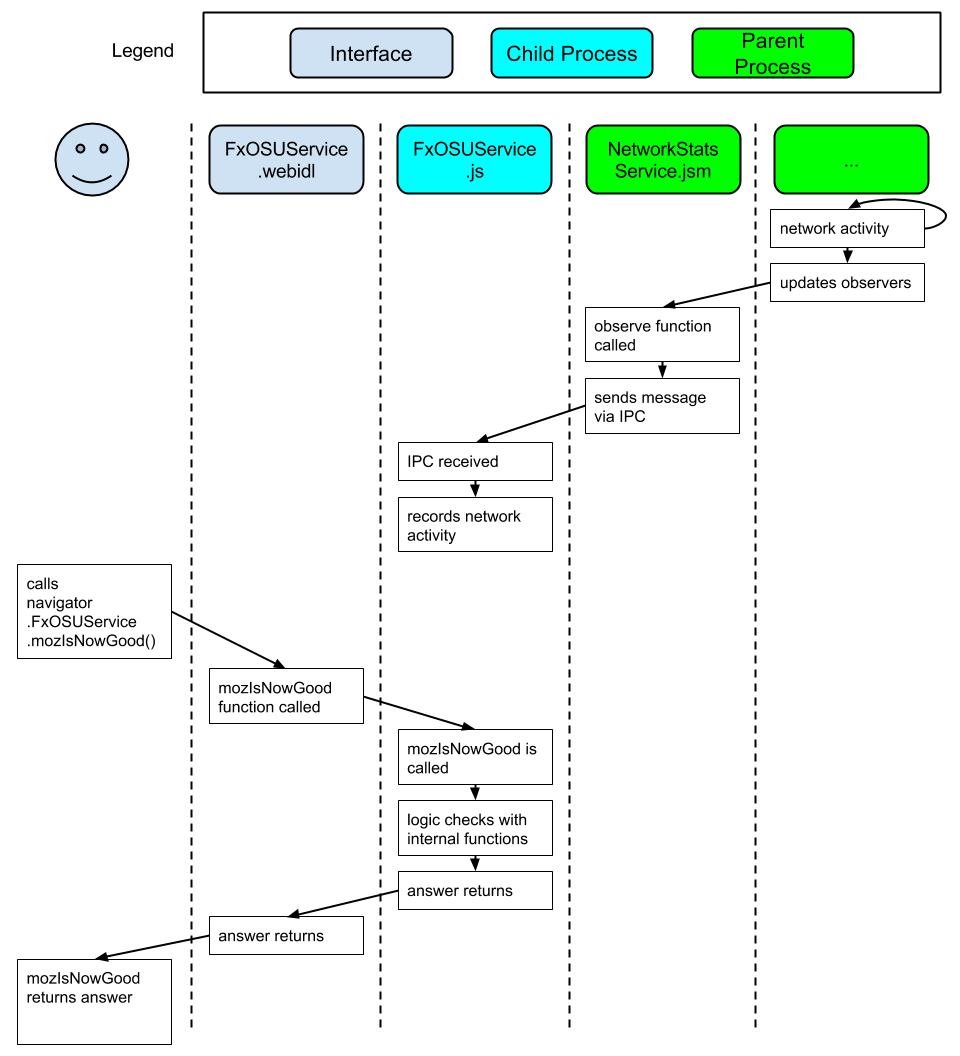
\includegraphics[scale=0.35]{userflow.png}
  \caption{Operational flow after a user calls the web-facing API.}
\end{figure}
\pagebreak

In some arbitrary developers application, there is a loop setup, calling our function periodically. The API is hanging off of the navigator object built into the browser, attached to our API service called 'FxOSUService'. When the application calls to receive a go/no-go answer, it calls navigator.FxOSUService.mozIsNowGood(), and waits for an answer. When the API is called, Firefox checks the webidl implementation to see what mozIsNowGood is. It finds out that it should return a boolean value, that it accepts an optional float value, and furthermore, the XPCOM component where the function lives. Once Firefox learns all of this, it calls the mozIsNowGood function in the XPCOM component. From here the mozIsNowGood function checks to see if a user specified level of confidence has been supplied, and if not, defaults the level to 2, which stands for moderate confidence level. From here mozIsNowGood calls its' internal functions (many of which are also exposed by the webidl), and obtains the device battery level, battery charging state, the connection stability, and connection success rate.
\\\\
With this data, the function moves into a switch/case which reads the confidence level, and from there checks against a number of evaluations based on the retrieved data, and if the data falls below the thresholds specified in that confidence level, then the function returns false, for no-go. However, if all evaluations pass without falling below a threshold specified by the confidence level, then the function returns true, for go. From here, the boolean answer is then returned back through the call chain setup from user, to webidl, to XPCOM component, and the call to navigator.FxOSUService.mozIsNowGood() returns a boolean go/no-go.

\subsection{Source Code}
Here is a description of each of the files used in our project.

\subsubsection{b2g/installer/package-manifest.in}
This file required modification to include references to our new XPCOM component. This is necessary when compiling Firefox OS; B2G (Boot 2 Gecko) contains the core which we continually refer to as Gecko.

\subsubsection{browser/installer/package-manifest.in}
This file required modification to include references to our new XPCOM component. This is necessary when compiling Firefox Desktop.

\subsubsection{dom/apps/PermissionsTable.jsm}
This file required modification to list the specific permissions given to the XPCOM component.

\subsubsection{dom/fxosu/FxOSUService.js}
This file holds the bulk of the work that we've done in this project. The work can be divided into two main parts.  There are a couple of global functions and variable which are used for IPC from NetworkStatsService.js and a prototype of our XPCOM Component called FxOSUService.  A subset of the functions in this prototype are then exposed as navigator properties.  These can be seen in FxOSUService.webidl section below.  Here are function prototypes for this file as well as brief descriptions as to what they do.
\\\\
\textbf{Global Functions}
\begin{itemize}
  \item \begin{lstlisting}[language=JavaScript]
importFactory(contractIdentification, interfaceName)
    \end{lstlisting}
    This function returns either an instance of an XPCOM component or a reference so and XPCOM service.  It is used internally by our Service to retrieve various XPCOM services which we need data from such as the Memory Reporter Manager and Network Link Service.  \\ 
  \item \begin{lstlisting}[language=JavaScript]
receiveMessage(aData)
    \end{lstlisting}
    This function is used to pass information between processes in the browser.  Our service uses this to receive messages from the Network Statistics Service to get information on recent network requests preformed on the device.  Unfortunately, at this point Network Statistics Service is only available on Firefox OS. 
\end{itemize}

\textbf{FxOSUService Functions}
\begin{itemize}
  \item \begin{lstlisting}[language=JavaScript]
FxOSUService.init()
    \end{lstlisting}  
    This function is automatically called upon application startup.  It is used to register observers for memory pressure events.  These allow our service to be notified when the device has an allocation failure or is running low on memory.  \\
  \item \begin{lstlisting}[language=JavaScript]
FxOSUService.observe(aSubject, aTopic, aData)
    \end{lstlisting} 
    This is the internal function used by the XPCOM observers service to provide notifications for registered observers. For example, when a low memory event occurs.  This function would be invoked by the observer service with a topic of "memory pressure".  This then allows our Service to record when the event occurred and what the current memory usage is.  We also get notified when the browser is shutting down so that we can clean up. \\
  \item \begin{lstlisting}[language=JavaScript]
FxOSUService.MemoryManager()
    \end{lstlisting} 
    This function calls the Memory Reporter XPCOM service to see what the current memory usage is.  It returns a dictionary containing the current Explicit and Resident memory usage numbers (in bytes).  Explicit memory usage is the amount of memory that has been explicitly allocated by calls to malloc or new.  Resident memory usage is the amount of physical memory is being used on the device by Firefox.  \\
  \item \begin{lstlisting}[language=JavaScript]
FxOSUService.numRequests(lastMillisecs)
    \end{lstlisting}  
    This function retrieves and counts the number of network requests that have been made in lastMillisecs milliseconds.  It is used internally to determine the success rate of network requests over a period of time.  
  \item \begin{lstlisting}[language=JavaScript]
FxOSUService.numResposes(lastMilisecs)
    \end{lstlisting} 
    This function retrieves and counts the number of network responses have been received in lastMillisecs milliseconds.  It is used internally to determine the success rate of network requests over a period of time.
  \item \begin{lstlisting}[language=JavaScript]
FxOSUService.receivedBytes(lastMillisecs)
    \end{lstlisting}
    This function returns the number of Bytes received in lastMillisecs milliseconds.  It is used internally to determine how much recent network activity there has been.  
  \item \begin{lstlisting}[language=JavaScript]
FxOSUService.successRate(lastMillisecs)
    \end{lstlisting}
    Returns a dictionary object that holds the success rate, \# of successes, and number of attempts for the lastMillisecs milliseconds.  It is used internally to determine the quality of the network over a period of time
  \item \begin{lstlisting}[language=JavaScript]
FxOSUService.successRateRecent(num)
    \end{lstlisting}
    Returns a dictionary object that holds the success rate, \# of successes, and number of attempts for the last num number of requests. It is used internally to determine the quality of the network for a specific group of requests.
  \item \begin{lstlisting}[language=JavaScript]
FxOSUService.IsConnectionStable(lastMillisecs)
    \end{lstlisting}
    This function returns a boolean value corresponding to whether the network has been stable over lastMillisecs milliseconds. A "Stable" connection is determined by no network requests failing over that period of time.  
  \item \begin{lstlisting}[language=JavaScript]
FxOSUService.batterylevel()
    \end{lstlisting}
    Returns the device's current battery level as a float value between 0 and 1.  
  \item \begin{lstlisting}[language=JavaScript]
FxOSUService.batterycharging()
    \end{lstlisting}
    Returns a boolean corresponding to whether the device is currently charging.  
  \item \begin{lstlisting}[language=JavaScript]
FxOSUService.latencyInfo()
    \end{lstlisting}
    Returns a dictionary object with latency times (in ms) for various stages of the request cycle as described in section 5.3.8
  \item \begin{lstlisting}[language=JavaScript]
FxOSUService.connectionType()
    \end{lstlisting}  
    Was supposed to use the Network Link Service to return the type of network (be in wifi, LTE, 3G, etc) But the functionality was intentionally disabled for security reasons.  At this time is returns 0 for LINK\_TYPE\_UNKNOWN. 
  \item \begin{lstlisting}[language=JavaScript]
FxOSUService.connectionUp()
    \end{lstlisting}
    Returns a boolean value corresponding to whether or not the device is currently has an active network connection. 
  \item \begin{lstlisting}[language=JavaScript]
FxOSUService.mozIsNowGood(level)
    \end{lstlisting}
    The primary function for our service which uses the device data we have access to using the functions above which provides a boolean interpreted as a go or no-go for three different levels of certainty about a network quality. Level 1 (highest) requires that no network requests have failed recently and that the device is currently plugged in.  Level 2 (moderate) returns false if the battery is not charging, the connection is not stable and the battery level is less than 40\% or if the battery is not charging and the battery is less than 30\% or if the success rate or recent network requests is less than 50\%. Level 3 (low) returns false if the connection is not stable and the battery is less than 20\% or if the battery is less than 10\% or if the success rate of recent requests is less than 5\%.
\end{itemize}

\subsubsection{dom/fxosu/FxOSUService.manifest}
This file sets the uuid for our XPCOM component, so that Gecko can handle a unique reference to the location of the component. It also sets up a name for the XPCOM component, and registers the component to be run at app startup.

\subsubsection{dom/fxosu/moz.build}
This file lists references to the files need to compile our XPCOM component, and is used by subsequent moz.build files up the directory hierarchy, when Gecko is being built.

\subsubsection{dom/NetworkStatsService.jsm}
This file required modification to handle registering network request observers, as well as handling the IPC functionality needed to shuttle messages from the parent process to a child process, and back again if necessary.
\\\\
We setup observers for 'http-on-modify-request' and 'http-on-examine-response' events. An 'http-on-modify-request' event is called whenever an http request is made. Among other things, this event allows you to inspect request headers and to even add or modify new and existing headers before the request is sent. An 'http-on-examine-response' event is called whenever a response has been received from the web server. Similarly to an 'http-on-modify-request' event, this event allows you to inspect response headers, and to modify existing response headers as well.
\\\\
Once the event observers are setup and registered, we define new cases for the NetworkStatsService.jsm process' observe function to be capable of reacting to our new events. Upon receipt of an 'http-on-modify-request' event, the observe function will grab the request URI and record the current time, storing this data in an object. This object is then broadcast asynchronously, with the name "NetworkStatsService:Request", where our FxOSUService.js child process is listening to grab the message. Upon receipt of an 'http-on-examine-response' event, the observe function will grab the content length in bytes, the time of the response, the content type, the response URI, will check if the response was a cached response by calling the isNoCacheResponse() function on the response object, and finally will check if the request succeeded by checking the requestSucceeded attribute of the response object. Just like with the 'http-on-modify-request' event, all of this data is then stored in an object, and the object is then broadcast asynchronously, with the name "NetworkStatsService:Response", where our FxOSUService.js child process is listening to grab the message.
\\\\
Finally, when the 'xpcom-shutdown' event is received, the observe function will remove the observers that we setup for 'http-on-modify-request' and 'http-on-examine-response' events.

\subsubsection{dom/webidl/FxOSUService.webidl}
This file handles the defining of our exposed API. In it we define the interface that will be made accessible via the navigator object available in a js application running in a web context. We define 3 objects to help with the interface we have chosen to implement; SuccessRateObject, MemoryObject, and LatencyObject. The SuccessRateObject object holds 3 floats; rate, successes, and attempted, which records the success rate from 0 to 1 of network requests, the number of successful network requests, and the total number of attempted network requests all within an arbitrary time period, respectively. The MemoryObject object holds 2 floats; explicit and resident. Explicit shows the total size of explicit memory allocations, both at the operating system level (mmap, VirtualAlloc) and at the heap level (malloc(), calloc(), operator new). And Resident shows the resident size (RSS) of physical memory used. The LatencyObject object holds 23 floats, which we'll list and describe in a bullet point list:

\begin{itemize}
  \item \textbf{navigation\_type}: the type of last non-redirect navigation
  \item \textbf{navigation\_redirectCount}: number of redirects since the last non-redirect navigation
  \item \textbf{prep}: the time taken from the first HTTP redirect starts to the prompt for unload the previous document
  \item \textbf{redirect}: the time taken for the last HTTP redirect
  \item \textbf{unload}: the time taken to complete the load event of the previous document
  \item \textbf{r\_to\_f}: the time taken from the start of resources fetching to the end of last HTTP redirect
  \item \textbf{fetch}: the time taken from the end of resources fetching to the start of domain name lookup
  \item \textbf{dnslookup}: the time taken to finish domain name lookup
  \item \textbf{d\_to\_c}: the time taken from the end of domain name lookup to the start of server connection
  \item \textbf{connection}: the time taken to establish connection to the server to retrieve the document 
  \item \textbf{c\_to\_req}: the time taken from finished connecting to the server to start requesting document from the server
  \item \textbf{request}: the time taken from the start of document request to the time when the user agent received the first byte of the response from the server
  \item \textbf{response}: the time taken from the user agent received the first byte of the response to the time the user agent received the last byte of the response from the server
  \item \textbf{res\_to\_dom}: the time taken from the user agent to receive the last byte of the response from the server to the time when user agent starts parsing the HTML document
  \item \textbf{domLoading}: the time taken for the user agent to finish parsing all the HTML document
  \item \textbf{domInteractive}: the time taken from the HTML document parsing finished to the time when script parsing starts
  \item \textbf{domContentLoaded}: the time taken for the user agent to finish parsing all the script
  \item \textbf{domComplete}: the time taken from the script parsing finished to the time when all the resources finished loading
  \item \textbf{dom\_to\_onload}: the time taken from all the resources finished loading to the time when load event starts
  \item \textbf{loadEvent}: the time taken to complete the load event of the current document
  \item \textbf{networkLatency}: the time taken from the start of resources fetching to the end of receiving data from the server
  \item \textbf{pageLoadingTime}: the time taken from the end of receiving data from the server to the end of loading the document
  \item \textbf{totalTimeElapsed}: the total time taken for the user agent to request and load the resources from the server
\end{itemize}

Finally, the WebIDL sets up 12 API functions that can be called from a web context, attached to navigator:
\begin{itemize}
  \item \textbf{boolean batteryLevel()}: Returns the battery level as a value between 0.0 and 1.0
  \item \textbf{boolean batteryCharging()}: Returns true if the battery is charging, otherwise false
  \item \textbf{DOMRequest recentRxTx()}: Returns a DOMRequest object describing the network statistics
  \item \textbf{float receivedBytes(optional float lastMillisecs)}: Returns the amount of data received, measured in bytes
  \item \textbf{SuccessRateObject successRate(optional float lastMillisecs)}: Returns a SuccessRateObject mentioned above
  \item \textbf{LatencyObject latencyInfo()}: Returns a LatencyObject mentioned above
  \item \textbf{boolean isConnectionStable(optional float lastMillisecs)}: Returns a Boolean value indicating the stableness of current connection
  \item \textbf{MemoryObject memoryManager();}: Returns a MemoryObject mentioned above
  \item \textbf{float connectionType()}: Returns a value from 0 to 7 indicating the current connection type such as Ethernet, WiFi and 4G
  \item \textbf{boolean connectionUp()}: Returns true if network is connected, otherwise false
  \item \textbf{float connectionQuality()}: Returns a float range from 0 to 1 which indicates the quality of current connection, where 0 is the worst and 1 is the best
  \item \textbf{boolean mozIsNowGood(optional float level)}: Takes a integer value of 1, 2 or 3 which represents the levels of certainty and returns a Boolean value indicating whether it is a good time to make a network request
\end{itemize}

\subsubsection{dom/webidl/moz.build}
This file lists references to the WebIDL files need to compile all API interfaces used in Firefox, and is used by subsequent moz.build files up the directory hierarchy, when Gecko is being built.

\subsubsection{dom/moz.build}
This file lists references to interfaces and the directory names of all XPCOM components stored in the dom/ directory, and is used by subsequent moz.build files up the directory hierarchy, when Gecko is being built.

\subsubsection{mobile/android/installer/package-manifest.in}
This file required modification to include references to our new XPCOM component. This is necessary when compiling Firefox for Android.
\pagebreak

\subsection{Building/Running from Source}
Running our project requires building a custom version of Firefox for the destination platform.  Our code 
functions on Firefox for Desktop, Firefox for Android as well as Firefox OS.  These build instruction are
written assuming you are using a Linux distribution (mostly for consistency). Building for Firefox OS is not currently supported in Windows. If your preferred OS is not Linux there will be links in the useful links section which will have instructions for Windows and Macintosh. 
\subsubsection{Linux Distribution Requirements}
	\begin{enumerate}
		\item 64 bit OS
		\item GCC 4.7 or later (4.8 for Firefox OS)
		\item 8GB of RAM is recommended (although not required)
		\item If you are compiling in a VM be sure to have at least 60GB of disk space (or more).
		\item I'd recommend a wired internet connection as well
	\end{enumerate}
\subsubsection{Install Build Prerequisites}
	\begin{enumerate}
	\item \textbf{Android/Desktop} \\
	If you want to build our code for Android or Desktop. Install these packages.  If you are trying to
	build Firefox OS skip to the next section which will be described in the next section. For Android or 
	Desktop the required packages can be installed using a Mozilla provided bootstrap file.  Run the
	wget command.  
	
	\begin{lstlisting}[style=BashInputStyle, breaklines=true]
	wget -q https://hg.mozilla.org/mozilla-central/raw-file/default/python/mozboot/bin/bootstrap.py && python bootstrap.py
	\end{lstlisting}

	You will be prompted whether you are trying to build for Desktop or Android. Select the build configuration you are  		attempting.  Note you can switch build platforms by running bootstrap again and re-configuring your .mozconfig file.  Note that bootstrapping for Android will take longer as it will install the entire Android platform.
	\item \textbf{Firefox OS}\\
	The prerequisites for building Firefox OS vary depending on the distribution of Linux that you are running as well as device you are targeting.  For these build instruction I am going to provide instructions for building on Ubuntu 12.04 targeting the Flame. The Flame is the official reference device for testing and debugging on Firefox OS.  We were provided with three of the devices for the year for testing/debugging.  
	
	If you are a using a different distribution or want to build for a different device instructions for getting the build prerequisites can be found here: \\ \\
	\href{https://developer.mozilla.org/en-US/Firefox\_OS/Firefox\_OS\_build\_prerequisites}{https://developer.mozilla.org/en-US/Firefox\_OS/Firefox\_OS\_build\_prerequisites}
	\begin{itemize}
		\item Install Ubuntu 12.04 Prerequisites (FIREFOX OS BUILDS ONLY) \\
		\begin{lstlisting}[style=BashInputStyle, breaklines=true]
sudo apt-get update
sudo apt-get install autoconf2.13 bison bzip2 ccache curl flex gawk gcc g++ g++-multilib git ia32-libs lib32ncurses5-dev lib32z1-dev libasound-dev libgconf2-dev libgl1-mesa-dev libx11-dev lzop make zip
sudo apt-get install libxml2-utils
			\end{lstlisting}
		\item Install adb (if you haven't already done so with the bootstrap command above) \\ \\
		There are many ways to install adb, the easiest is on Ubuntu 12.04 is to download and extract the Android SDK found here.\\ \\
		\href{http://developer.android.com/sdk/installing/index.html}{http://developer.android.com/sdk/installing/index.html}
		\item Configure udev rules for the device \\ \\
		This can be done by adding the following lines to your /etc/udev/rules.d/android.rules file.  NOTE: if this file doesn't exist you should create it and use chmod to make it readable.  
	\begin{lstlisting}[style=BashInputStyle, breaklines=true]
SUBSYSTEM=="usb", ATTR{idVendor}=="05c6", MODE="0666", GROUP="plugdev"
SUBSYSTEM=="usb", ATTR{idVendor}=="18d1", MODE="0666", GROUP="plugdev"
	\end{lstlisting}
		After adding the rules restart the udev daemon
		\begin{lstlisting}[style=BashInputStyle]
sudo service udev restart
		\end{lstlisting}	
	\end{itemize}
	\end{enumerate}	

\subsubsection{Get a Copy of Mozilla Central}
	Run the following command to checkout a copy of Mozilla Repository.  This could take awhile (depending 
	on your internet connection.)  There is a LOT of code!
	
	\begin{lstlisting}[style=BashInputStyle, breaklines=true]
	hg clone https://hg.mozilla.org/mozilla-central
	\end{lstlisting}
	
\subsubsection{Get a Copy of our Source} 
	While you have been given our source code, the easiest way to get our code in place in our copy of mozilla-central is by
	checking out a copy of our repository. 

	\begin{lstlisting}[style=BashInputStyle, breaklines=true]
	hg clone https://github.com/JohnLZeller/fxosu.git
	\end{lstlisting}	
	
\subsubsection{Patching Our Code into Mozilla Central}
	Getting our source code positioned in mozilla-central to be built is simple using mercurial.  Navigate to the mozilla-
	central directory which was created a two steps ago.  Use the following command replacing the path with the path to the
	diff file which is inside the repository for our source which was created last step.
	
	\begin{lstlisting}[style=BashInputStyle]
	hg import path/to/fxosu.diff
	\end{lstlisting}
	
\subsubsection{Building and Running Firefox!}
	\begin{enumerate}
		\item \textbf{Desktop} \\ \\
		For desktop no build configurations are required.  To build our code navigate to the mozilla-central directory and run
\begin{lstlisting}[style=BashInputStyle]
./mach build
./mach run
\end{lstlisting}
The final command should launch the newly built Firefox Browser with our service built it!
		\item \textbf{Android} \\ \\
		Android requires configuring to build depending on the target device.  	This is done using a configuration file called .mozconfig in the root of the mozilla-central directory.  This file is automatically generated for building desktop.  But requires some options to configure the build for android.  Create a .mozconfig text file and add the following options:
		
		\begin{lstlisting}[style=BashInputStyle]
# Build Firefox for Android:
ac_add_options --enable-application=mobile/android

# Chose one of the following for targets for x86 or ARM
ac_add_options --target=i386-linux-android
ac_add_options --target=arm-linux-androideabi

# With the following Android SDK and NDK:
ac_add_options --with-android-sdk="/path/to/android-sdk/platforms/android-22"
ac_add_options --with-android-ndk="/path/to/android-ndk-r10e"
		\end{lstlisting}
Be sure to only include one of the --target options above depending on the architecture of your device or emulator. After creating the configuration file the following commands will build, package and install Firefox to you device.  Make sure that your device is plugged in and connected to adb before running these commands. 
\begin{lstlisting}[style=BashInputStyle]
./mach build
./mach package
./mach install
\end{lstlisting}
		\item \textbf{Firefox OS}
		\begin{itemize}
		\item Clone the B2G (Boot 2 Gecko) repository.  \\
		This is done using git.
\begin{lstlisting}[style=BashInputStyle]
git clone git://github.com/mozilla-b2g/B2G.git
\end{lstlisting}
		\item Navigate to the repository
\begin{lstlisting}[style=BashInputStyle]
cd B2G
\end{lstlisting}
		\item Create a .userconfig file \\
		We are doing this because we want to build with the custom version on mozilla-central we created in the last couple of steps.  Create a file called .userconfig in the B2G directory and add the following lines replacing the paths with the path to our custom mozilla-central repository.
\begin{lstlisting}[style=BashInputStyle]
export GECKO_PATH=/path/to/mozilla-central
export GECKO_OBJDIR=/path/to/mozilla-central/objdir-gonk
\end{lstlisting}
		\item Configure for the Flame \\
\begin{lstlisting}[style=BashInputStyle]
./config.sh flame-kk
\end{lstlisting}
		\item Build!
\begin{lstlisting}[style=BashInputStyle]
./build.sh
\end{lstlisting}
		\item Flash onto the Device
\begin{lstlisting}[style=BashInputStyle]
./flash.sh
\end{lstlisting}
		\end{itemize}
		\end{enumerate}
		
\subsubsection{Running Our Test Application}
Once you have built for any of the platforms testing our application running our test application is as simple as opening the  web browser you just built and navigate to: \\ (\href{http://ivantjiam.github.io/fxosu-test/}{http://ivantjiam.github.io/fxosu-test/}). 
\subsubsection{Running Our API in the Web Console}
It is also possible to run functions in our API via the Web Console.  For Android and Firefox OS this requires use of the Firefox WebIDE. WebIDE did not begin supporting Firefox for Android until Firefox 36.  Getting this version may require updating Firefox on your distribution.  
\begin{enumerate}
\item \textbf{Desktop} \\
Running our API in Firefox for Desktop is as simple as pressing \keys{F12} or \keys{\ctrl + \shift + k} and typing any of the functions listed in the Webidl file described earlier. 
\item \textbf{Android} \\
To open WebIDE open Firefox on your host device and press \keys{\shift + f8}. 
To run our API first you must get your Device/Emulator connected as a runtime to the host machine running Firefox 36 or later.  To do so 
\begin{enumerate}
\item Connect the Device to the host machine 
\item Enable Remote Debugging on the Device or Emulator
\item Enable Remote Debugging in Firefox for Android 
\item Connect to the device in WebIDE 
\end{enumerate}
\begin{center}
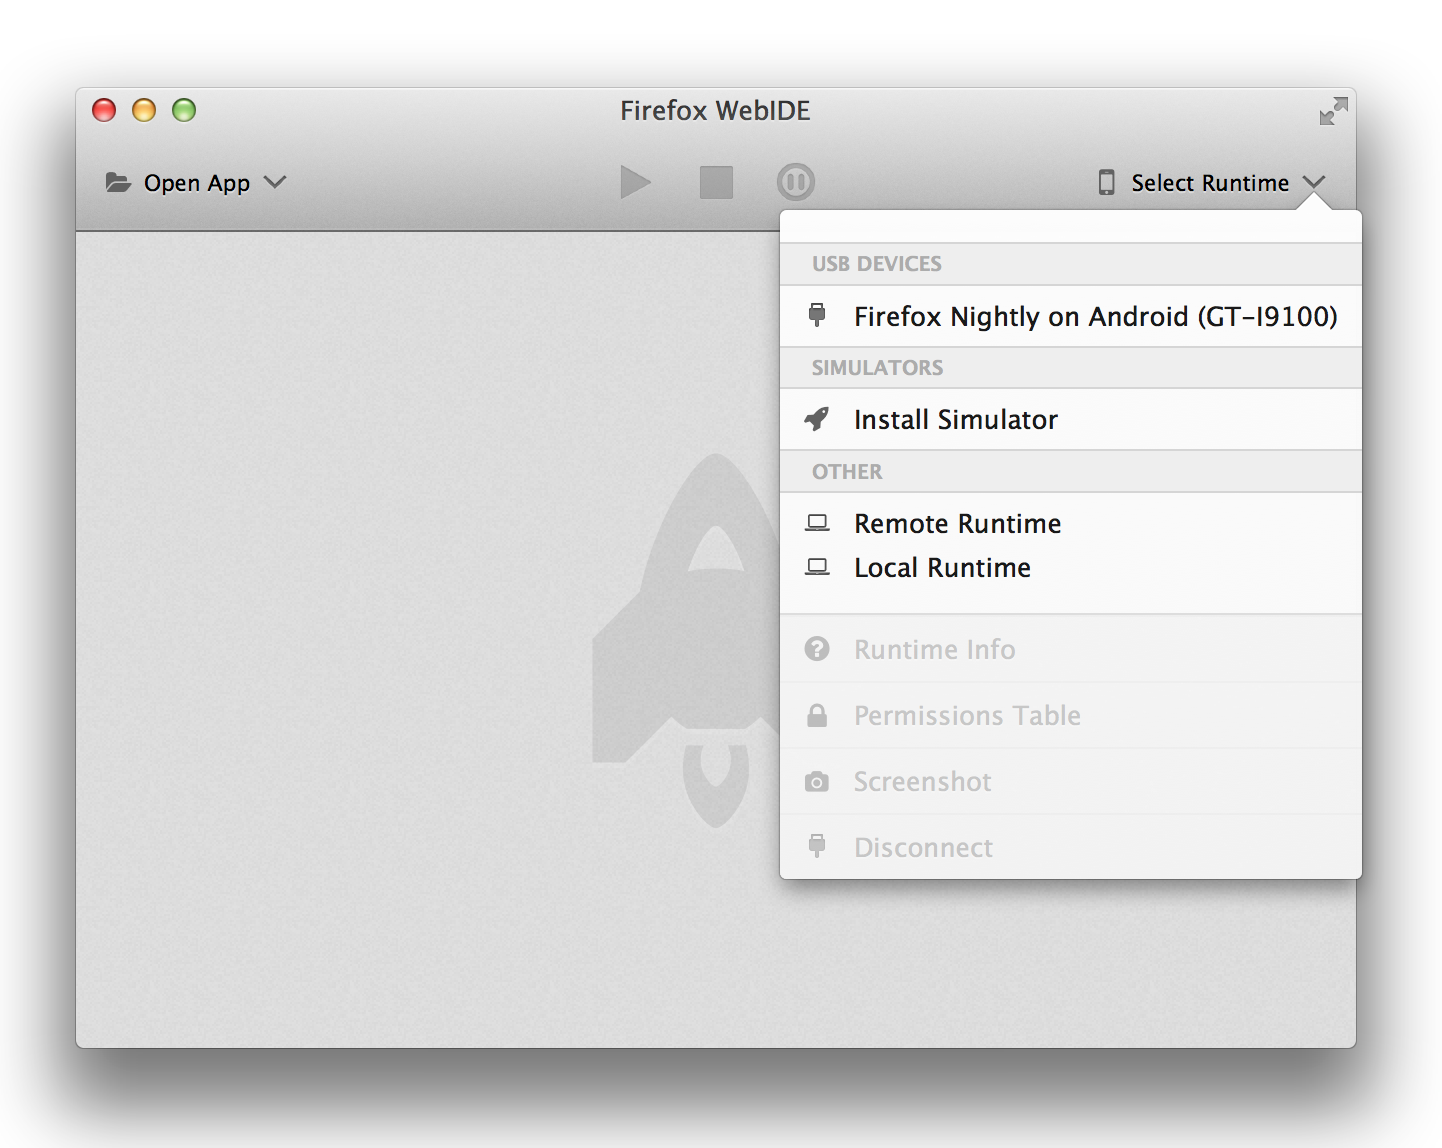
\includegraphics[scale=0.4]{remote-debugging-android-runtime} \\
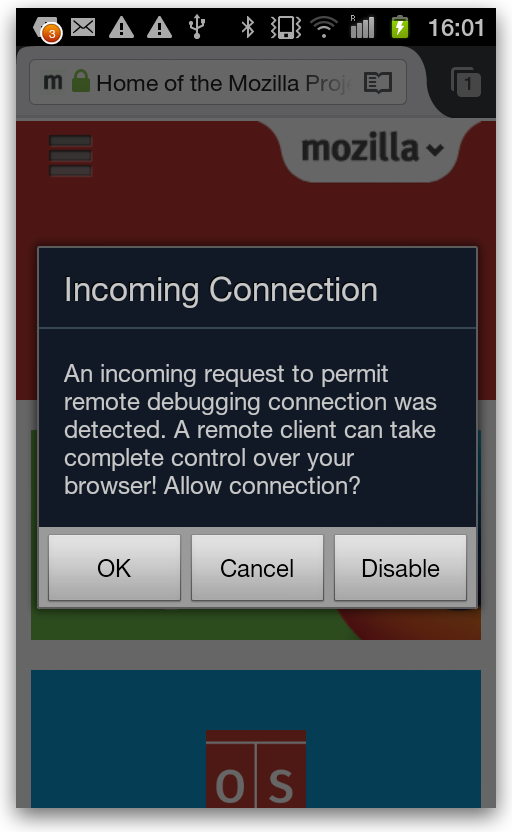
\includegraphics[scale=0.25]{incoming-warning} \\
The Device will prompt you about an incoming connection. Click OK \\
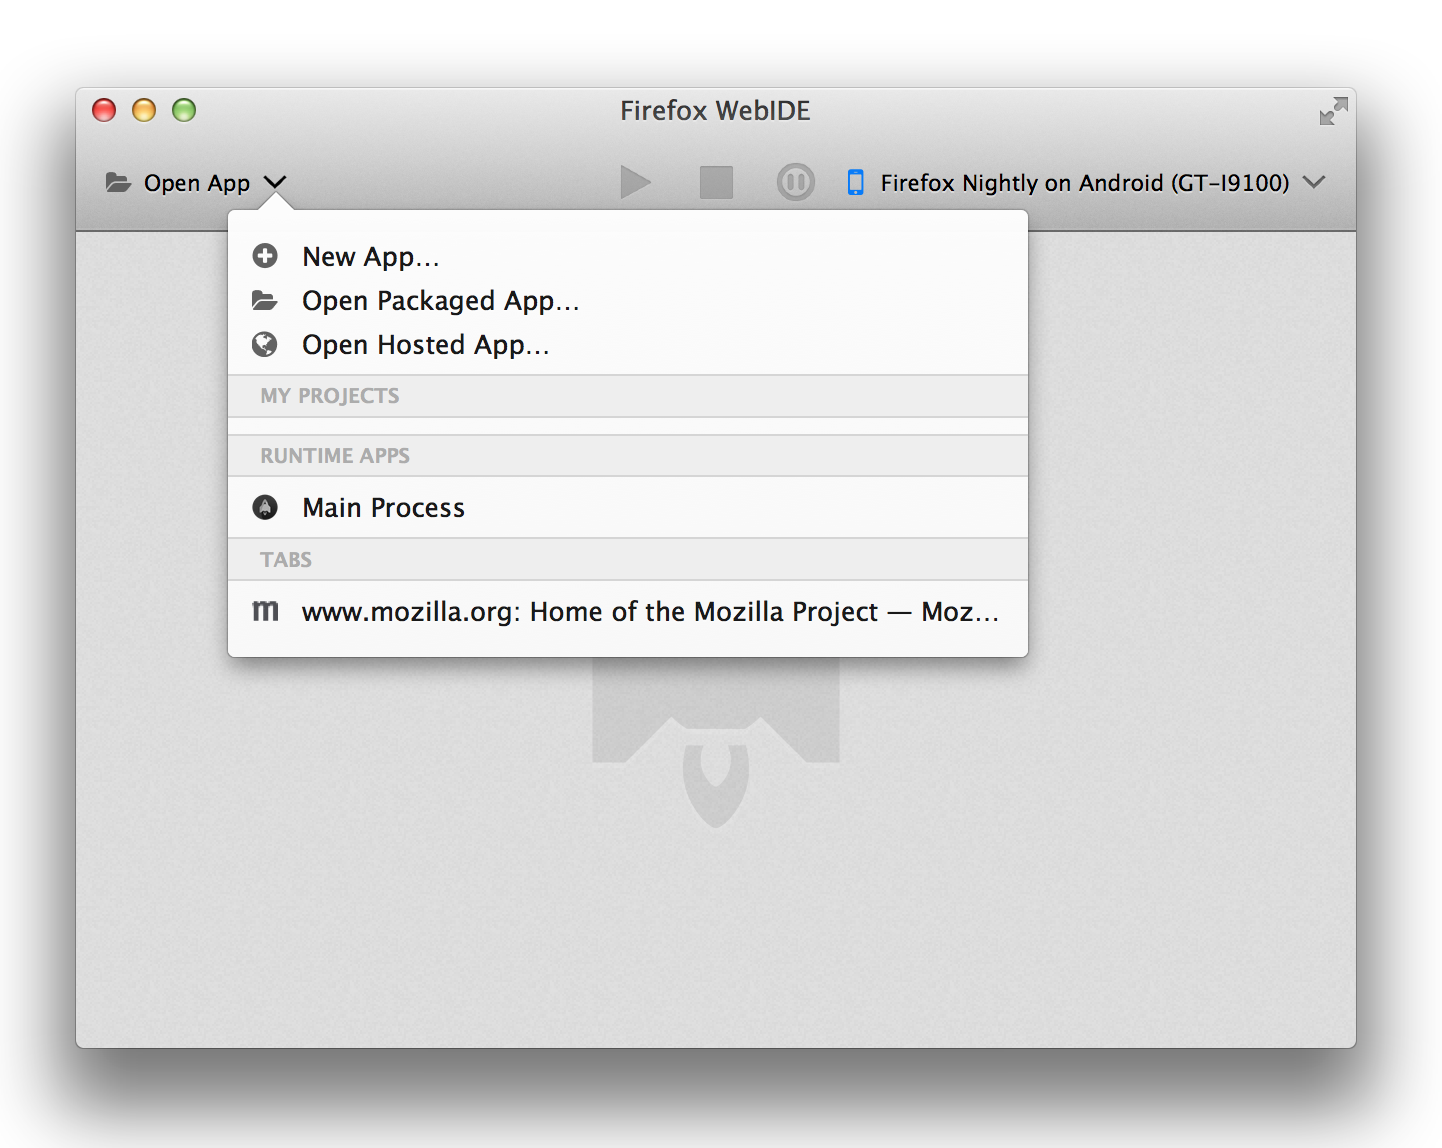
\includegraphics[scale=0.4]{remote-debugging-android-open-tabs} \\
After the connection has been established clicking the Open App tab in WebIDE should display all of the open tabs on the device.
Selecting any of these tabs will allow you to run any of the functions listed in our Webidl file above on the devices Web console. 
\end{center}
\item \textbf{Firefox OS} \\
The process is largely the same for Firefox OS as it is for Android
\begin{enumerate}
\item Connect the Device to the host machine
\pagebreak
\item Enable Remote Debugging on the Device \\ \\
In Firefox OS this can be done in the developers panel. You may have to enable the panel by navigating to: 
\menu{Settings > Device information > More Information > Developer Menu Checkbox}. You can then access
the developers men via \menu{Settings > Developer} to enable remote debugging.  \\ \\
\begin{center}
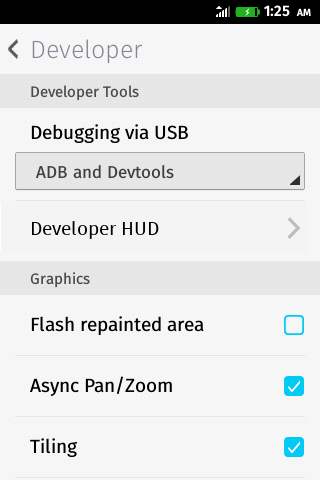
\includegraphics[scale=0.5]{developermenu-short} \\
Be sure to enable for both adb and DevTools
\end{center}
\item Connect to the Device in WebIDE
\end{enumerate}
\end{enumerate}
\pagebreak

\subsection{API Documentation}
The functionality of our API has been heavily documented in Section 5.3.4 in the Source Code section.

\pagebreak

\section{Learning New Technology}
% What web sites were helpful? (Listed in order of helpfulness.)
% What, if any, reference books really helped?
% Were there any people on campus that were really helpful? 
There were a number of websites that were helpful during the course of researching, designing, implementing and testing our project. Here is a list of the websites that we found most useful, organized from most to least helpful:
\begin{enumerate}
	\item Mozilla Developer Network\\ (\href{https://developer.mozilla.org/en-US/}{https://developer.mozilla.org/en-US/})
	\item Mozilla Wiki\\ (\href{https://wiki.mozilla.org/}{https://wiki.mozilla.org/})
	\item Boot2Gecko Mailing List\\ (\href{https://groups.google.com/forum/\#!forum/mozilla.dev.b2g}{https://groups.google.com/forum/\#!forum/mozilla.dev.b2g})
	\item Gaia Mailing List\\ (\href{https://groups.google.com/forum/\#!forum/mozilla.dev.gaia}{https://groups.google.com/forum/\#!forum/mozilla.dev.gaia})
	\item StackOverflow\\ (\href{http://stackoverflow.com/}{http://stackoverflow.com/})
	\item W3Schools\\ (\href{http://www.w3schools.com/js/}{http://www.w3schools.com/js/}) 
	\item Mozilla Cross Reference\\ (\href{http://mxr.mozilla.org/}{http://mxr.mozilla.org/})
\end{enumerate}
	

And here are a list of webpages, within these websites that we found most useful, organized from most to least helpful:
\begin{enumerate}
	\item MDN XPCOM Interface Reference\\ (\href{https://developer.mozilla.org/en-US/docs/Mozilla/Tech/XPCOM/Reference/Interface}{https://developer.mozilla.org/en-US/docs/Mozilla/Tech/XPCOM/Reference/Interface})
	\item MDN Building Firefox OS\\ (\href{https://developer.mozilla.org/en-US/Firefox\_OS/Building\_and\_installing\_Firefox\_OS}{https://developer.mozilla.org/en-US/Firefox\_OS/Building\_and\_installing\_Firefox\_OS})
	\item MDN Building Firefox Desktop \\(\href{https://developer.mozilla.org/en-US/docs/Mozilla/Developer\_guide/Build\_Instructions}{https://developer.mozilla.org/en-US/docs/Mozilla/Developer\_guide/Build\_Instructions})
	\item Mozilla Wiki Building Firefox for Android \\ (\href{https://wiki.mozilla.org/Mobile/Fennec/Android}{https://wiki.mozilla.org/Mobile/Fennec/Android})
	\item MDN Observer Notifications \\ (\href{https://developer.mozilla.org/en-US/docs/Observer\_Notifications}{https://developer.mozilla.org/en-US/docs/Observer\_Notifications})
	\item MDN WebIDE \\(\href{https://developer.mozilla.org/en-US/docs/Tools/WebIDE}{https://developer.mozilla.org/en-US/docs/Tools/WebIDE})
	\item MDN XPCOM Reference for nsIMemoryReporterManager \\ (\href{https://developer.mozilla.org/en-US/docs/Mozilla/Tech/XPCOM/Reference/Interface/nsIMemoryReporterManager}{https://developer.mozilla.org/en-US/docs/Mozilla/Tech/XPCOM/Reference/\\Interface/nsIMemoryReporterManager})
\end{enumerate}

\noindent Other resources that we found really helpful included:
\begin{enumerate}
	\item IRC (irc.mozilla.org)
		\subitem Find more info here: \href{https://wiki.mozilla.org/IRC}{https://wiki.mozilla.org/IRC}
\end{enumerate}
\pagebreak

\section{What did we learn from all of this?}
\subsection{John Zeller}
\textbf{What technical information did you learn?}\\
I learned a lot about JavaScript. When I first began working on this project, I came in with the urge to do and learn something outside of my comfort zone. I usually write in Python, and have primarily used Python in the 3 internships that I have had. So, writing JavaScript, and moreover, becoming acquainted with Firefox source code were both amazing learning experiences.
\\\\
Digging into the Firefox source code gave me a much better idea of how a browser is put together. Understanding the complexities of a relatively small part of Firefox, such as IPC, has given me a great insight into the complexity of this code base.
\\\\
\textbf{What non-technical information did you learn?}\\
I learned more about the organization of teams within Mozilla, and the separation of efforts in one product, across multiple teams. There really is a huge amount of institutional knowledge, and a lot of it has been written out in their wiki pages. I also learned that a lot of those wiki pages are out of date, and need some love.
\\\\
\textbf{What have you learned about project work?}\\
I learned a lot about the importance of a design cycle such as Agile. Most of the senior design process is sort of intrinsically setup in a Waterfall design cycle, but you are free to iterate on that, running your own weekly, bi-weekly, monthly etc. Agile cycles. Our group in particular ran into this pretty hard, and we ended up changing 10 of our 24 requirements. When we originally wrote our requirements document during Fall term, we had an idea of what the project would look like, and not 4 weeks later, that idea changed significantly.
\\\\
\textbf{What have you learned about project management?}\\
Other than the importance of design cycles, as I mentioned above, I learned about the importance of constant communication with your project customer. It's very possible that the ideas you have begun to spin within your own mind, and in the hive mind of the project group, could be wildly different, or even slightly misaligned from that of the project customer, and the much larger hive mind of your customers organization. 
\\\\
\textbf{What have you learned about working in teams?}\\
I've certainly learned about the importance of communication throughout the project. Often we would run into issues where one or more of our group members were lost, while perhaps at least one knew the way forward. Clear communication and clearing up questions is something that produces a well oiled machine.
\\\\
\textbf{If you could do it all over, what would you do differently?}\\
If I could do it all over again, I would spend significantly more time researching our project during October, before our requirements document was written. If we were able to have overcome many of the changes that we needed to make later on, this would have seriously increased the ease of implementation that we experienced throughout the project.
\\
\pagebreak
\subsection{Pok Yan Tjiam}
\textbf{What technical information did you learn?}\\
I learned the architecture of Firefox OS and other technologies that may seems useful such as ServiceWorker and XPCOM. I also learned how to write API in JavaScript and how to develop Firefox add-on. Since I never use JavaScript before, it took me some time to get familiar with it.
\\\\
\textbf{What non-technical information did you learn?}\\
I learned where to find information for writing web API. Mozilla Developer Network, Mozilla wiki and W3C specification contains many useful information about web API.
\\\\
\textbf{What have you learned about project work?}\\
I learned the importance and usefulness of version control. We use GitHub for version control, backup and code sharing. It keeps track of every change we made to the code and helps us manage our code.
\\\\
\textbf{What have you learned about project management?}\\
Time management is critical to a project's success. There was a few times we fall behind the schedule due to coursework from other classes. Sometimes a bug just took too long to solve. The project could run smoother if we can better estimate the time for each tasks.
\\\\
\textbf{What have you learned about working in teams?}\\
Communication is very important. To create a successful team, we have to make sure everyone is on the same page, keep track of each other's progress and share each other's opinion for improvement. It is important to have weekly meetings with team members to discuss the current progress of the project and solve problems together.
\\\\
\textbf{If you could do it all over, what would you do differently?}\\
If I could do it all over, I would spend more time on the implementation and testing on Firefox OS device instead of Firefox desktop. Although Firefox OS and Firefox desktop share the same core, some of the functions and APIs only work on Firefox OS. If we focus on Firefox OS, we can spend less time on writing unused code and rewriting functions.
\\
\pagebreak
\subsection{Jonathan McNeil}
\textbf{What technical information did you learn?} \\
I was very new to front end technology at the beginning of the project.  Most of my experience here at Oregon State as well as
in the work force was in lower level languages such like C and C++. This project gave me a chance to learn and use Javascript, HTML and CSS.  One of the most intriguing things that I learned was how to implement functionality that can be used cross-platform using XPCOM. 
\\\\
\textbf{What non-technical information did you learn?}\\
Interacting with our client as well as people on IRC taught me a lot about the software development process in an open source community like Mozilla.  This was a very different experience for me.  People were always willing to help when I ran into a problem all I had to do was hop into an IRC channel and ask my question.  I often times wouldn't even be asking the right questions and yet still would come away with the answer I was looking for. I also learned some of the flaws of the open source community.  The biggest example being the lack of good documentation (or horrifically out of date documentation).  The best bet was looking at actual source code or asking questions in IRC.  
\\\\
\textbf{What have you learned about project work?}\\
I learned that a project with a goal this big only gets done in increments.  It is not
like a homework assignment for a class where often times you can sit down and get the majority of the work done 
in a sitting.  This project required large amounts of research and time to even sit down and write a line of code.  Getting even the simplest things working can take a lot of time. I also learned the importance of stepping away when you get stuck.  There were several times when I would get stuck on a bug and would end up getting frustrated and wasting time.  It was far more worthwhile to step away and work on something else and come back to the problem later. 
\\\\ 
\textbf{What have you learned about project management?}\\
I learned that over the course of a long project like this it is important to be flexible.  During the fall we got a broad view of what we thought the client was looking for out of this project. But during the Winter when we met with him up in Portland we discovered that what we had envisioned wasn't what he was looking for.  When designing software you need to be flexible and ready for things to change.
\\\\\\
\textbf{What have you learned about working in teams?}\\
Communication is vital. We were only able to meet face to face a couple times a week which made those times extremely important. We needed to work out what progress was made as well as what needed to get done next.  This wasn't always simple as what we were working on could depend on something that another team member was working on.  Having to balance project work with work from other classes also made it important to communicate when you could or could not work on the project.  I found that the less we talked, the less that seemed to get done during that period of time.  Constant communication led to more efficient work which led to more progress.   
\\\\
\textbf{If you could do it all over, what would you do differently?}\\
If I was going to do it all over I would of spent a lot more time and effort during the fall term during the research phase.  We met with our client and got an idea of what he was looking for. We had to change several requirements because once we started putting in some time we realized that our idea wasn't correct.  If we had spent more time and effort researching and communicating with our client we could have realized this sooner which would of made the implementation process a lot easier.  
\pagebreak

\appendix
\section{Appendix I}
% Essential Code Listings. You don't have to include absolutely everything, but if someone wants to understand your project, there should be enough here to learn from. If you worked within a larger project, something like a patch file might be a good way to go.
\subsection{API Source Code}
Full up-to-date source code can be found at: \href{https://github.com/JohnLZeller/fxosu}{https://github.com/JohnLZeller/fxosu}

\subsubsection{b2g/installer/package-manifest.in}
\lstinputlisting[language=diff, breaklines=true]{diffs/b2g-installer-package-manifest.diff}
\pagebreak

\subsubsection{browser/installer/package-manifest.in}
\lstinputlisting[language=diff, breaklines=true]{diffs/browser-installer-package-manifest.diff}
\pagebreak

\subsubsection{dom/apps/PermissionsTable.jsm}
\lstinputlisting[language=diff, breaklines=true]{diffs/dom-apps-PermissionsTable.diff}
\pagebreak

\subsubsection{dom/fxosu/FxOSUService.js}
\lstinputlisting[language=javascript, breaklines=true]{source/FxOSUService.js}
\pagebreak

\subsubsection{dom/fxosu/FxOSUService.manifest}
\lstinputlisting[breaklines=true]{source/FxOSUService.manifest}
\pagebreak

\subsubsection{dom/fxosu/moz.build}
\lstinputlisting[breaklines=true]{source/dom-fxosu-moz.build}
\pagebreak

\subsubsection{dom/NetworkStatsService.jsm}
\lstinputlisting[language=diff, breaklines=true]{diffs/dom-network-NetworkStatsService.diff}
\pagebreak

\subsubsection{dom/webidl/FxOSUService.webidl}
\lstinputlisting[language=javascript, breaklines=true]{source/FxOSUService.webidl}
\pagebreak

\subsubsection{dom/webidl/moz.build}
\lstinputlisting[language=diff, breaklines=true]{diffs/dom-webidl-moz.diff}
\pagebreak

\subsubsection{dom/moz.build}
\lstinputlisting[language=diff, breaklines=true]{diffs/dom-moz.diff}
\pagebreak

\subsubsection{mobile/android/installer/package-manifest.in}
\lstinputlisting[language=diff, breaklines=true]{diffs/mobile-android-installer-package-manifest.diff}
\pagebreak

\subsection{Test App Source Code}
Full up-to-date source code can be found at: \href{https://github.com/IvanTjiam/fxosu-test}{https://github.com/IvanTjiam/fxosu-test}

\subsubsection{index.html}
\lstinputlisting[language=html, breaklines=true]{source/testapp/index.html}
\pagebreak

\subsubsection{manifest.webapp}
\lstinputlisting[language={}, breaklines=true]{source/testapp/manifest.webapp}
\pagebreak

\subsubsection{js/app.js}
\lstinputlisting[language=javascript, breaklines=true]{source/testapp/app.js}
\pagebreak

\subsubsection{js/filter.js}
\lstinputlisting[language=javascript, breaklines=true]{source/testapp/filter.js}
\pagebreak

\subsubsection{css/app.css}
\lstinputlisting[language={}, breaklines=true]{source/testapp/app.css}
\pagebreak

\section{Appendix II}
% Anything else you want to include. Photos, etc.
\subsection{Glossary}
\textbf{Gecko}: the layout engine developed by the Mozilla Project, originally named NGLayout. Gecko reads web content, such as HTML, CSS, XUL, JavaScript, and renders it on the user's screen. In XUL-based applications, Gecko is used to render the application's user interface as well.\\(\href{https://developer.mozilla.org/en-US/docs/Mozilla/Gecko}{https://developer.mozilla.org/en-US/docs/Mozilla/Gecko})
\\\\
\textbf{IPC}: inter-process communication; the activity of sharing data across multiple and commonly specialized processes using communication protocols.\\(\href{http://en.wikipedia.org/wiki/Inter-process_communication}{http://en.wikipedia.org/wiki/Inter-process\_communication})
\\\\
\textbf{JSM}: a JavaScript Code module. It lets multiple privileged JavaScript scopes share code. For example, a module could be used by Firefox itself as well as by extensions, in order to avoid code duplication.\\(\href{https://developer.mozilla.org/en-US/docs/Mozilla/JavaScript_code_modules}{https://developer.mozilla.org/en-US/docs/Mozilla/JavaScript\_code\_modules})
\\\\
\textbf{MDN}: Mozilla Developer Network\\(\href{https://developer.mozilla.org/en-US/}{https://developer.mozilla.org/en-US/})
\\\\
\textbf{Necko}: a network library that provides a platform-independent API for several layers of networking, ranging from transport to presentation layers. This API is used in many Mozilla-based client applications (including Firefox) and can be used for writing other networking clients.\\(\href{https://developer.mozilla.org/en-US/docs/Necko}{https://developer.mozilla.org/en-US/docs/Necko})
\\\\
\textbf{URI}: a uniform resource identifier is a string of characters used to identify a name of a resource.\\(\href{http://en.wikipedia.org/wiki/Uniform_resource_identifier}{http://en.wikipedia.org/wiki/Uniform\_resource\_identifier})
\\\\
\textbf{WebIDL}: a format for describing interfaces that are intended to be implemented in web browsers.\\(\href{http://en.wikipedia.org/wiki/Web_IDL}{http://en.wikipedia.org/wiki/Web\_IDL})
\\\\
\textbf{XPCOM}: a cross platform component object model, similar to Microsoft COM. It has multiple language bindings, allowing XPCOM components to be used and implemented in JavaScript, Java, and Python in addition to C++. Interfaces in XPCOM are defined in a dialect of IDL called XPIDL.\\(\href{https://developer.mozilla.org/en-US/docs/Mozilla/Tech/XPCOM}{https://developer.mozilla.org/en-US/docs/Mozilla/Tech/XPCOM})
\\\\
\textbf{Mozilla-Central}: The central Mercurial repository for all released code by Mozilla.\\(\href{https://developer.mozilla.org/en-US/docs/mozilla-central}{https://developer.mozilla.org/en-US/docs/mozilla-central})

\end{document}
